\documentclass[tikz,border=5pt]{standalone}
\usepackage{pgfplots}
\pgfplotsset{compat=1.18}

\definecolor{exponencial}{HTML}{C2415D}
\definecolor{polinomi}{HTML}{365FB3}
\definecolor{guia}{HTML}{6B7280}

\begin{document}
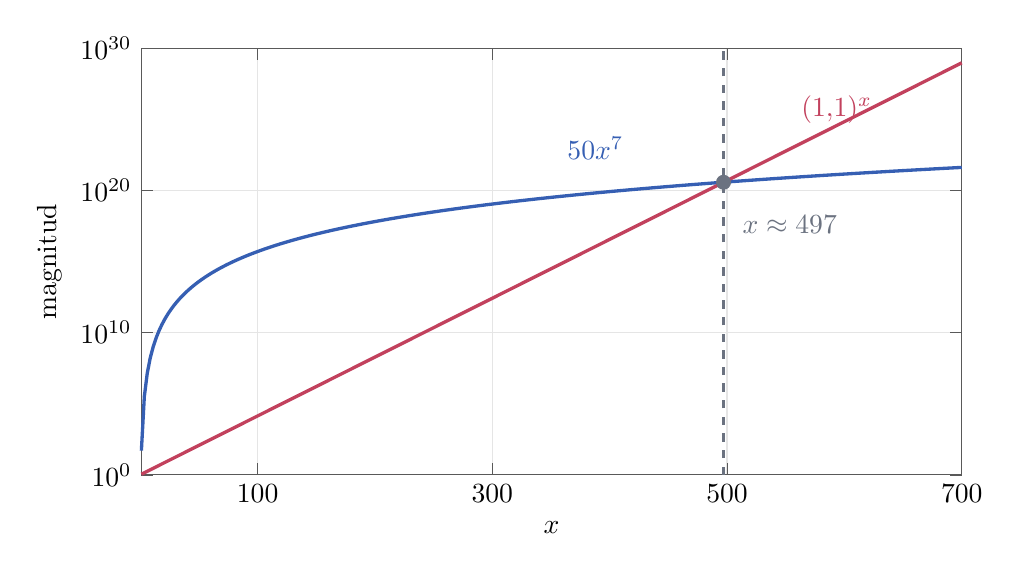
\begin{tikzpicture}
  \begin{axis}[
    width=12cm,
    height=7cm,
    xmin=1,
    xmax=700,
    ymin=1,
    ymax=1e30,
    ymode=log,
    log basis y=10,
    xlabel={$x$},
    ylabel={magnitud},
    xtick={100,300,500,700},
    ytick={1e0,1e10,1e20,1e30},
    yticklabels={$10^0$,$10^{10}$,$10^{20}$,$10^{30}$},
    axis line style={black!65},
    tick style={black!65},
    grid=major,
    grid style={black!10},
    clip=false,
  ]
    \addplot[polinomi, very thick, domain=1:700, samples=280]
      {50*x^7};
    \addplot[exponencial, very thick, domain=1:700, samples=280]
      {1.1^x};

    \addplot[guia, dashed, thick] coordinates {(497,1) (497,1e30)};
    \addplot[only marks, mark=*, mark size=2.5pt, guia]
      coordinates {(497,3.7e20)};

    \node[anchor=south east, text=polinomi]
      at (axis cs:420,3e21) {$50x^7$};
    \node[anchor=south west, text=exponencial]
      at (axis cs:555,1e24) {$(1{,}1)^x$};
    \node[anchor=north west, text=guia]
      at (axis cs:505,8e18) {$x\approx497$};
  \end{axis}
\end{tikzpicture}
\end{document}
